\chapter{Darko UAV modelling}
% \minitoc

\section{Model of the DarkO UAV}
\label{sec:model}
The DarkO UAV, designed and developed at the Ecole Nationale de l'Aviation Civile (ENAC) in Toulouse
 (France), is a clear example of a convertible UAV with a so-called tail-sitter architecture. 
 DarkO is assembled from multiple 3D printed Onyx parts (a highly robust material comprising 
 omnidirectional carbon fibres). All surfaces are interlocked on a single axis, so that the drone 
 can be easily disassembled for parts replacement or to gain access to the on-board electronics. 

The on-board autopilot is an Apogee~\footnote{\url{https://wiki.paparazziuav.org/wiki/Apogee/v1.00}} 
board manufactured at ENAC, see Fig. \ref{fig:apogee}. 
\begin{figure}[ht]
\centering
    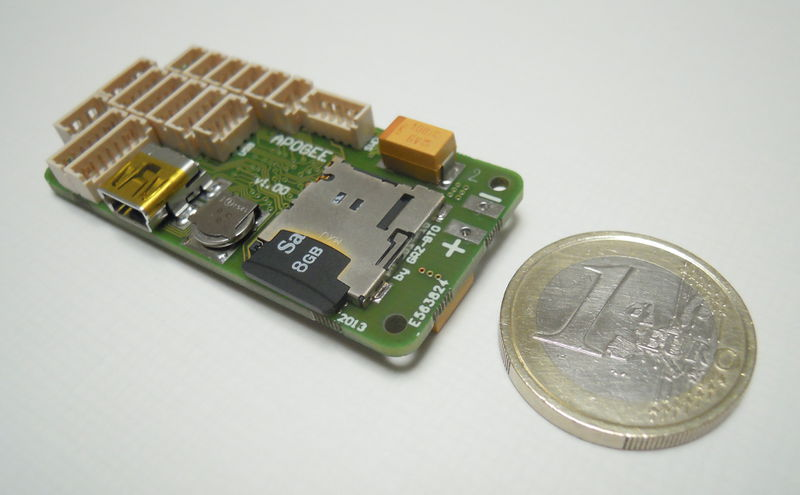
\includegraphics[width=0.8\columnwidth]{figures/800px-Apogee_v100_top_1E.jpeg}
    \caption{Apogee v1.00 top view.}
    \label{fig:apogee}
\end{figure}
The autopilot provides the option of recording the on-board data on an SD memory card, at the control
 frequency of 500 Hz, thus allowing for effective post-processing of acquired data. 
 The communication protocol used between the autopilot and the Electronic Speed Controllers (ESCs)
  is Dshot 600. The ESCs are AIKON AK32 35A flash with an AM32 firmware. The ground-to-board
   communication is performed via a bidirectional channel based on XBee-PRO S1 modules.
\begin{figure}[ht]
\centering
    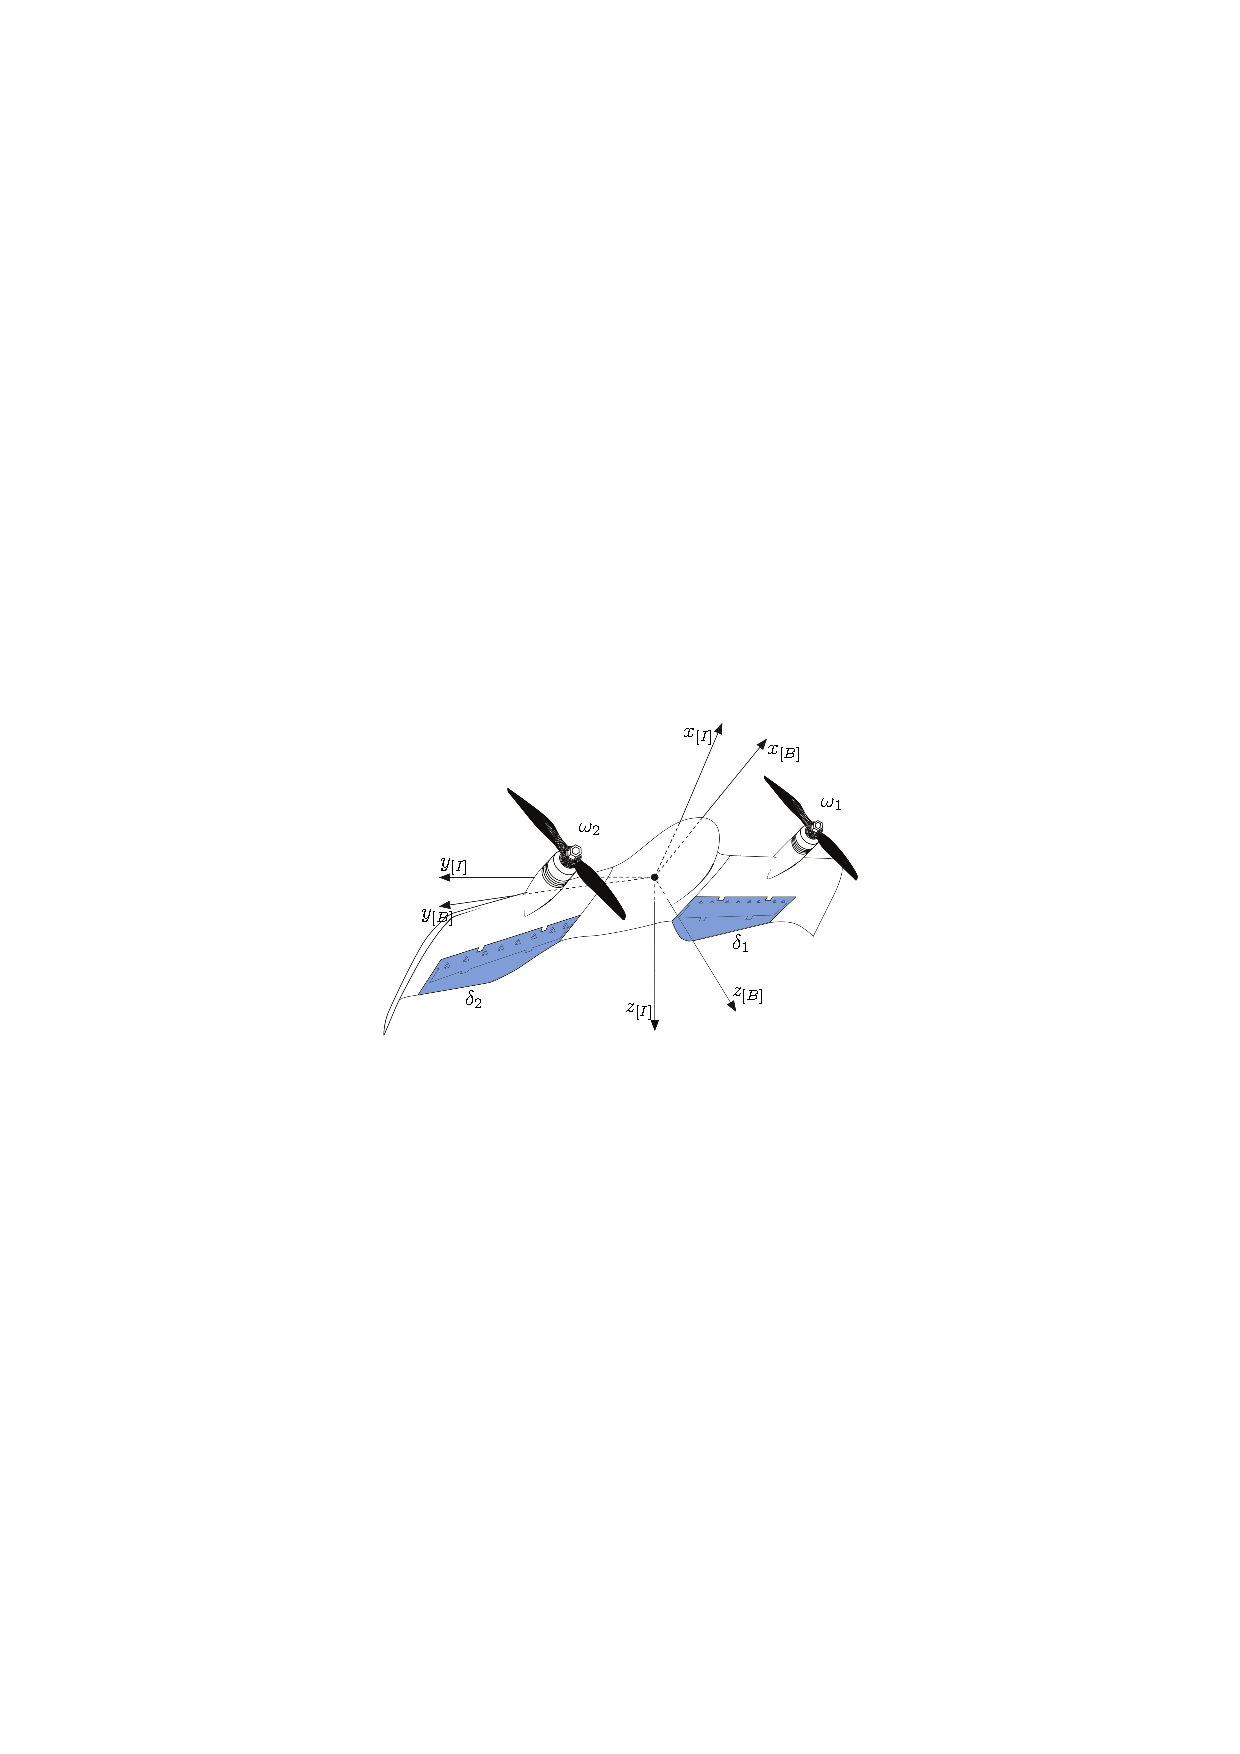
\includegraphics[width=1\columnwidth]{figures/darko.pdf}
    \caption{DarkO body frame with a schematic representation of the actuators.}
    \label{fig:darko2}
\end{figure}
DarkO's actuators consist in two propellers (T-Motor T5147) symmetrically placed at the front of the wing (shown in \textbf{black} in Fig. \ref{fig:darko2}) powered by two T-Motor F30 2300kv electric motors and two elevons, placed at the back of the wing (shown in \textcolor{cyan}{blue} in Fig. \ref{fig:darko2}) and acting as control surfaces. The elevons are driven by two MKS DS65K servomotors. Fig.~\ref{fig:darko2} shows the DarkO model, together with a NED inertial reference frame (or world frame) ``$\text{i}$'' linked to the Earth's surface,
and a body reference frame ``$\text{b}$'' attached to the drone, with $x_{\text{b}}$ corresponding to the roll axis (the propellers axe laying in the $z_{\text{b}} =0$ plane), $y_{\text{b}}$ the pitch axis (the direction of the wings), $z_{\text{b}}$ the yaw axis. Using the same notation as in \cite{lustosa:hal-03035938}, the left and right propeller/elevon are denoted by using subscripts $i=1$ (left) and $i=2$ (right). The sign convention will be defined positive for the elevons positions $\delta_{1}$, $\delta_{2}$ when they create a pitch-up moment with the propellers rotating in a opposite directions with angular speeds $\omega_{1} > 0 $ and $\omega_{2} < 0$, respectively.
\begin{table}[ht]
  \centering
    \begin{tabular}{|l|c|c|}
      \hline
      \multicolumn{1}{|c|}{Parameter or coefficient} & Value & Units  \\
      \hline
      $m$ (drone mass)  & 0.519 & \SI{}{\kilogram} \\
      \hline
      $b$ (wingspan)  & 0.542 & \SI{}{\meter} \\
      \hline
      $c$ (aerodynamic cord)  & 0.13 & \SI{}{\meter} \\
      \hline
      $\boldsymbol{B}=\diag(b,c,b)$ & $\!\!\diag(0.542, 0.13, 0.542)$ \!\! & \SI{}{\meter}\\
      \hline
      $S$ (wing area) & 0.026936 & \SI{}{\square\meter}\\
      \hline
      $S_{\text{wet}}$ (wet area) & 0.0180 & \SI{}{\square\meter}\\
      \hline
      $S_{\text{p}}$ (propeller area) & 0.0127 & \SI{}{\square\meter}\\
      \hline
      % $J_{x}$ & 0.0070 & \SI{}{\kilogram\square\meter}\\
      % \hline
      $\boldsymbol{J}=\diag(J_{x},J_{y},J_{z})$ & \!\! $\diag(0.0072,0.0004,0.0086)$\!\! & \SI{}{\kilogram\square\meter}\\
      % \hline
      % $J_{z}$ & 0.0061 & \SI{}{\kilogram\square\meter}\\
    %   \hline
    %   $J_{p}$ & 5.1116e-6 & \SI{}{\kilogram\square\meter}\\
      \hline
      $k_{\text{f}}$ (propeller thrust) & 1.7800e-8 & \SI{}{\kilogram\meter}\\
      \hline
      $k_{\text{m}}$(propeller torque) & 2.1065e-10 & \SI{}{\kilogram\square\meter}\\
      \hline
      $p_{x}$ (propeller $x$ location) & 0.065 & \SI{}{\meter}\\
      \hline
      $p_{y}$ (propeller $y$ location) & 0.162 & \SI{}{\meter}\\
      \hline
      $a_{y}$ (lift $y$ position) & 0.1504 & \SI{}{\meter}\\
      \hline
      $\xi_{\text{f}}$ (elevons lift) & 0.2 & --\\
      \hline
      $\xi_{\text{m}}$ (elevons torque) & 1.4 & --\\
      \hline
      $\rho$ (air density) & 1.225 & \SI{}{\kilogram\per\cubic\meter}\\
      \hline
      $C_{\text{d}}$ (drag coefficient) & 0.1644 & --\\
      \hline
      $C_{y}$ (lateral coefficient) & 0 & --\\
      \hline
       $C_{\ell}$ (lift coefficient) & 5.4001 & --\\
      \hline
      $\Delta_{\text{r}}$ (UAV centering) & -0.0145 & \SI{}{\meter}\\
      \hline
    \end{tabular}
    \caption{\label{tab:pars} Identified numerical parameters of the DarkO model.}
\end{table}

\subsection{Full nonlinear model}

Exploiting the modelling reported in \cite{lustosa:hal-03035938} and \cite{olszaneckibarth:hal-02542982}, an accurate model of the DarkO dynamics describes the position $\boldsymbol{p} \in \real^3$ of the origin of the body frame  and its velocity $\boldsymbol{v} = \dot{\boldsymbol{p}} \in \real^3$, in addition to its orientation, well represented by a quaternion $\boldsymbol{q} \in {\mathbb S}^3:=\{ \boldsymbol{q}\in \real^4: |\boldsymbol{q}| = 1\}$ and its angular velocity $\boldsymbol{\omega}_{\text{b}}$ represented in the body frame, which satisfies
$\boldsymbol{\dot q} = \frac{1}{2}\boldsymbol{q} \otimes \smallmat{0 \\ \boldsymbol{\omega}_{\text{b}}}$, where $\otimes$ denotes the quaternion product (see \cite{lustosa:hal-03035938,olszaneckibarth:hal-02542982} or the tutorial \cite{hamel_minhduc} for the details).
Selecting the overall state as $\boldsymbol{x}:=(\boldsymbol{p},~ \boldsymbol{v},~ \boldsymbol{q},~  \boldsymbol{\omega}_{\text{b}})$, the mathematical model derived in \cite{lustosa:hal-03035938}, depend on a set of parameters listed in Table \ref{tab:pars}, where we also report the value obtained from a system identification \cite{sansou:stage}. The dynamic model can be written as
\begin{subequations}\label{eq:dyna_orig}
  \begin{empheq}[left=\empheqlbrace]{alignat=2}
        % \boldsymbol{\dot p} & &= & \boldsymbol{v} \label{eq:dyna1}\\
        m\boldsymbol{\dot v} &&=& - m\boldsymbol{g} +  \boldsymbol{R}(\boldsymbol{q})\boldsymbol{F}_{\text{b}},\\
        \label{eq:dyna_orig_b}
        \boldsymbol{J} \boldsymbol{\dot \omega_{\text{b}}} &&= &  - \skewsym{\boldsymbol{\omega}_{\text{b}}}\boldsymbol{J}\boldsymbol{\omega}_{\text{b}} + \boldsymbol{M}_{\text{b}},
  \end{empheq}
\end{subequations}
where $\boldsymbol{g}:=\smallmat{0 & 0& 9.81}^\top$ denotes the gravity vector, $m\in \real$ is the mass, $\boldsymbol{J}\in \real^{3\times 3}$ is the diagonal moment of inertia (see Table~\ref{tab:pars}) and, partitioning the quaternion $\boldsymbol{q} \in {\mathbb S}^3$ as $\boldsymbol{q} := \left [ \eta ~ \boldsymbol{\epsilon}^\top \right]^\top$, the corresponding rotation matrix $\boldsymbol{R}(\boldsymbol{q}) \in SO(3): = \{\boldsymbol{R}\in \real^{3\times 3}: \; \boldsymbol{R}^\top \boldsymbol{R} = \mathbb{I}_{3}, \det (\boldsymbol{R})=1\}$ is defined as (see \cite{hamel_minhduc})
\begin{align}
    \label{eq:matrix_rot}
    \boldsymbol{R}(\boldsymbol{q}) := \mathbb{I}_{3} +2\eta \skewsym{\boldsymbol{\epsilon}} + 2\skewsym{\boldsymbol{\epsilon}}^{2}.
\end{align}
According to \cite{lustosa:hal-03035938} the force and moment vectors $\boldsymbol{F}_{\text{b}}$ and $\boldsymbol{M}_{\text{b}}$ in \eqref{eq:dyna_orig} depend on (i) the state $\boldsymbol{x}$, (ii) the disturbance $\boldsymbol{w} \in \real^3$, representing the wind speed in the world frame, and (iii) the actuators commands (see Figure~\ref{fig:darko2}), comprising the two propellers' rotational speeds
$\omega_1, \omega_2 \in \real$ and the two elevons' deflections $\delta_1, \delta_2\in \real$.
Let us first consider the actuators commands' effect. Each propeller generates a thrust $\boldsymbol{T}_i$ oriented in the $x$ direction of the body frame and a moment $\boldsymbol{N}_i$ about the same axis:
\begin{align}
\label{eq:thrust}
\boldsymbol{T}_{i} \!:=\! \begin{bmatrix} \tau_{i} \\ 0 \\ 0 \end{bmatrix} \!:=\!
\begin{bmatrix} k_{\text{f}}\omega_{i}^{2} \\ 0 \\ 0 \end{bmatrix}\! , \;
\boldsymbol{N}_{i} \!:=\! (-1)^{i}  \frac{k_{\text{m}} }{k_{\text{f}}}\boldsymbol{T}_{i}, \quad i=1,2 .
\end{align} 
Each elevon's position $\delta_i \in \real$ is assigned by a servo-motor that imposes an efficiency level (in terms of airstream deflection) quantified by two skew-symmetric matrices:
\begin{align}
\label{eq:elevons_efficiency}
    \boldsymbol{\Delta}^{\text{f}}_{i} \!:=\! \begin{bmatrix} 0 & 0 & \xi_{\text{f}}\delta_{i} \\ 0 & 0 & 0 \\ -\xi_{\text{f}}\delta_{i} & 0 & 0 \end{bmatrix}\! ,\;
    \boldsymbol{\Delta}^{\text{m}}_{i} \!:=\! \begin{bmatrix} 0 & 0 & \xi_{\text{m}}\delta_{i} \\ 0 & 0 & 0 \\ -\xi_{\text{m}}\delta_{i} & 0 & 0 \end{bmatrix} \!, 
\end{align}
$i=1,2$. The constant parameters $k_{\text{f}}$, $k_{\text{m}}$, $\xi_{\text{f}}$, $\xi_{\text{m}}$ appearing in \eqref{eq:thrust} and \eqref{eq:elevons_efficiency} are listed in Table~\ref{tab:pars}.\\
With the above actuation quantities, we may rearrange the dynamics given in \cite[eqns (97),~(98)]{lustosa:hal-03035938} (see also \cite{sansou:stage}) and express $\boldsymbol{F}_{\text{b}}$ and $\boldsymbol{M}_{\text{b}}$ in \eqref{eq:dyna_orig} as
%
\begin{align}
%\begin{split}
\nonumber
    \boldsymbol{F}_{\text{b}} :={}&  \boldsymbol{T}_{1} + \boldsymbol{T}_{2} + \frac{S_{\text{wet}}}{4S_{\text{p}}} \boldsymbol{\Phi}^{\text{(fv)}} \Big( (\boldsymbol{\Delta}^{\text{f}}_1 - \mathbb{I}_{3} ) \boldsymbol{T}_{1} + ( \boldsymbol{\Delta}^{\text{f}}_2 - \mathbb{I}_{3}) \boldsymbol{T}_{2}\Big) \\ 
     \label{eq:Fb}
    &+ \frac{1}{4} \rho S  \boldsymbol{\Phi}^{\text{(fv)}} \Big(\boldsymbol{\Delta}^{\text{f}}_1+ \boldsymbol{\Delta}^{\text{f}}_2 - 2 \mathbb{I}_{3} \Big) \lVert \boldsymbol{v_{\text{b}}} \rVert \boldsymbol{v_{\text{b}}}\\
    \nonumber
    &+ \frac{1}{4} \rho S \boldsymbol{\Phi}^{\text{(mv)}} \Big(\boldsymbol{\Delta}^{\text{f}}_1 + \boldsymbol{\Delta}^{\text{f}}_2 - 2\mathbb{I}_{3}\Big) \boldsymbol{B} \lVert \boldsymbol{v_{\text{b}}} \rVert  \boldsymbol{\omega}_{\text{b}}, 
%\end{split}
\end{align}
% 
\begin{align} 
\label{eq:Mb}
% \begin{split}
 \boldsymbol{M}_{\text{b}} :&=\boldsymbol{N}_{1} + \boldsymbol{N}_{2} + \skewsym{\smallm{p_x\\ p_y\\ 0}} \boldsymbol{T}_{1} + \skewsym{\smallm{p_x\\ - p_y\\ 0}} \boldsymbol{T}_{2}\\
    \nonumber
  &- \frac{S_{\text{wet}}}{4S_{\text{p}}} \bigg( \boldsymbol{B} \boldsymbol{\Phi}^{\text{(mv)}} (\boldsymbol{\Delta}^{\text{m}}_1- \mathbb{I}_{3} ) + \skewsym{\smallm{0 \\ a_y \\ 0}} \boldsymbol{\Phi}^{\text{(fv)}} (\boldsymbol{\Delta}^{\text{m}}_1 +\mathbb{I}_{3} ) \bigg) \boldsymbol{T}_{1} \\
    \nonumber
  & - \frac{S_{\text{wet}}}{4S_{\text{p}}} \bigg( \boldsymbol{B} \boldsymbol{\Phi}^{\text{(mv)}} (\boldsymbol{\Delta}^{\text{m}}_2 - \mathbb{I}_{3} ) +  \skewsym{\smallm{0 \\ - a_y \\ 0}} \boldsymbol{\Phi}^{\text{(fv)}} (\boldsymbol{\Delta}^{\text{m}}_2 + \mathbb{I}_{3}) \bigg) \boldsymbol{T}_{2} \\
    \nonumber
  & + \frac{1}{4} \rho S  \bigg( \Big(\skewsym{\smallm{0 \\ a_y \\ 0}} \!\!\! \boldsymbol{\Phi}^{\text{(fv)}}  + \boldsymbol{B} \boldsymbol{\Phi}^{\text{(mv)}} \Big) \boldsymbol{\Delta}^{\text{m}}_1 \\
    \nonumber
  &  + \Big( \skewsym{\smallm{0 \\ - a_y \\ 0}} \!\!\! \boldsymbol{\Phi}^{\text{(fv)}} + \boldsymbol{B} \boldsymbol{\Phi}^{\text{(mv)}}  \Big) \boldsymbol{\Delta}^{\text{m}}_2 - 2 \boldsymbol{B} \boldsymbol{\Phi}^{\text{(mv)}}  \bigg) \lVert \boldsymbol{v_{\text{b}}} \rVert \boldsymbol{v_{\text{b}}} \\
    \nonumber
  & +\frac{1}{4} \rho S \bigg(\!\! \Big(\!\! \skewsym{\!\smallm{0 \\ a_y \\ 0}\!}\!\!\! \boldsymbol{\Phi}^{\text{(mv)}} \! + \! \boldsymbol{B} \boldsymbol{\Phi}^{\text{(m$\omega$)}} \Big) \boldsymbol{\Delta}^{\text{m}}_1 \\
    \nonumber
  & +  \Big(\!\! \skewsym{\!\smallm{0 \\ - a_y \\ 0}\!} \!\!\! \boldsymbol{\Phi}^{\text{(mv)}} \! + \! \boldsymbol{B} \boldsymbol{\Phi}^{\text{(m$\omega$)}}  \Big) \boldsymbol{\Delta}^{\text{m}}_2 - 2 \boldsymbol{B} \boldsymbol{\Phi}^{\text{(m$\omega$)}}\!  \bigg)\!  \boldsymbol{B}  \lVert \boldsymbol{v_{\text{b}}} \rVert  \boldsymbol{\omega}_{\text{b}} ,
% \end{split}
\end{align}
where $\boldsymbol{v}_{\text{b}} := \boldsymbol{R}^\top(\boldsymbol{q}) (\boldsymbol{v}-\boldsymbol{w})$ represents the air speed seen by the drone, represented in the body frame. In \cite{lustosa:hal-03035938}, the scalars $\lVert \boldsymbol{v_{\text{b}}} \rVert$ appearing in the expressions of $\boldsymbol{F}_{\text{b}}$ and $\boldsymbol{M}_{\text{b}}$ are replaced by the scalar $\eta = \sqrt{\lVert \boldsymbol{v_{\text{b}}} \rVert^{2} + \mu c^{2} \lVert \boldsymbol{\omega}_{\text{b}} \rVert^{2}}$, with $\mu \in \real$ being a parameter related to the model identification, but in the case of DarkO \cite{sansou:stage}, the identification provides $\mu = 0$, therefore we present a simplified description here. The constant aerodynamic coefficients' matrix 
$\boldsymbol{\Phi}:= \begin{bmatrix} \boldsymbol{\Phi}^{\text{(fv)}} & {\boldsymbol{\Phi}^{\text{(mv)}}}^\top \\ \boldsymbol{\Phi}^{\text{(mv)}} & \boldsymbol{\Phi}^{\text{(m$\omega$)}} \end{bmatrix} \in \real^{6 \times 6}$, is defined in \cite[eqs. (6)--(9)]{olszaneckibarth:hal-02542982} as $ \boldsymbol{\Phi}^{\text{(fv)}} \!:=\! \diag(C_{\text{d}},C_{y}, C_{\ell})$ and
\begin{align*}
&\left[ \begin{array}{c|c}
    \boldsymbol{\Phi}^{\text{(mv)}}  &  \boldsymbol{\Phi}^{\text{(m$\omega$)}} 
\end{array}\right] :=\\ 
&\left[ \begin{array}{ccc|ccc}
    0 & 0 & 0    &                                          0.1396 & 0 & 0.0573 \\
    0 & 0 & \!\!\!\!\! -\frac{\Delta_{\text{r}}}{c}C_{\ell} &    0 &  0.6358  & 0 \\
    0 & 0 & 0 &     0.0405 & 0 & 0.0019 
\end{array}\right],
\end{align*}
the numerical values of the constants being reported in Table~\ref{tab:pars} (these numerical values were not reported in \cite{lustosa:hal-03035938} and \cite{olszaneckibarth:hal-02542982} and are given here to allow reproducing our simulation results). The numerical values in Table \ref{tab:pars} have been obtained by a model identification campaign \cite{sansou:stage}. In particuler, coefficient $k_{\text{f}}$ was identified from the equation \eqref{eq:thrust}, which links the motor rotation speed $\omega_{i}$ with the generated traction, the minimum and maximum rotation speed and the time constant of the motor actuation chain. The diagonal elemnts of the inertia $\boldsymbol{J}$ were measured using a bifilar pendulum system. This method is widely used in the drone field \cite{Jardin2007OptimizedMO}, and is based on the period of oscillation about each one of the three axes ($x_{\text{b}}$,$y_{\text{b}}$,$z_{\text{b}}$) of the drone suspended by two wires, which forms a torsion pendulum as shown in Fig. \ref{fig:BifilarPend}.
It is interesting to note that the surface area blown by the propellers represents 67 percent of the drone's total surface area.


\begin{figure}[ht!]
    \centerline{
    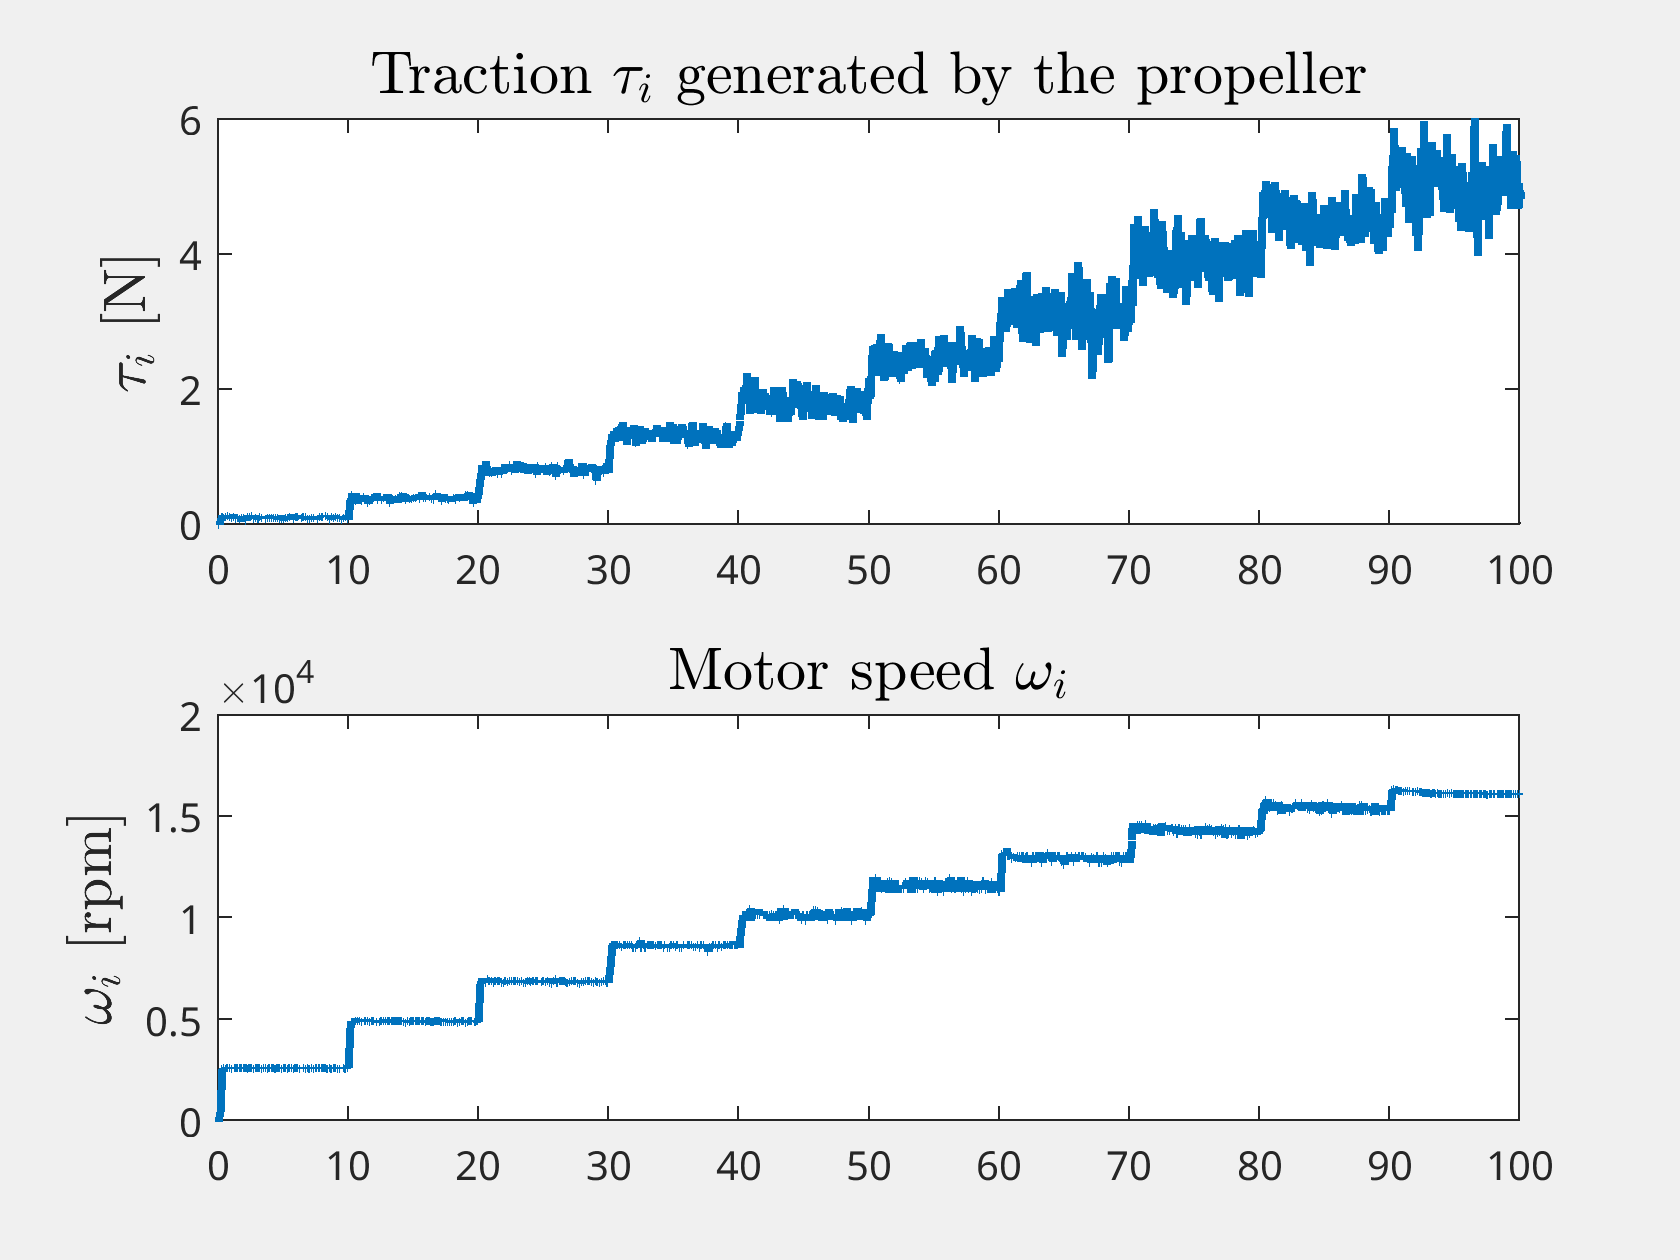
\includegraphics[trim=0cm 0cm 0cm 0cm,clip,width=1\columnwidth]{figures/ident_motor March 27 2024 1651.png}}
    \caption{Input-output response of an Esc-Motor-Propeller assembly.}
    \label{IOmot}
\end{figure}

\begin{figure}[ht!]
    \centerline{
    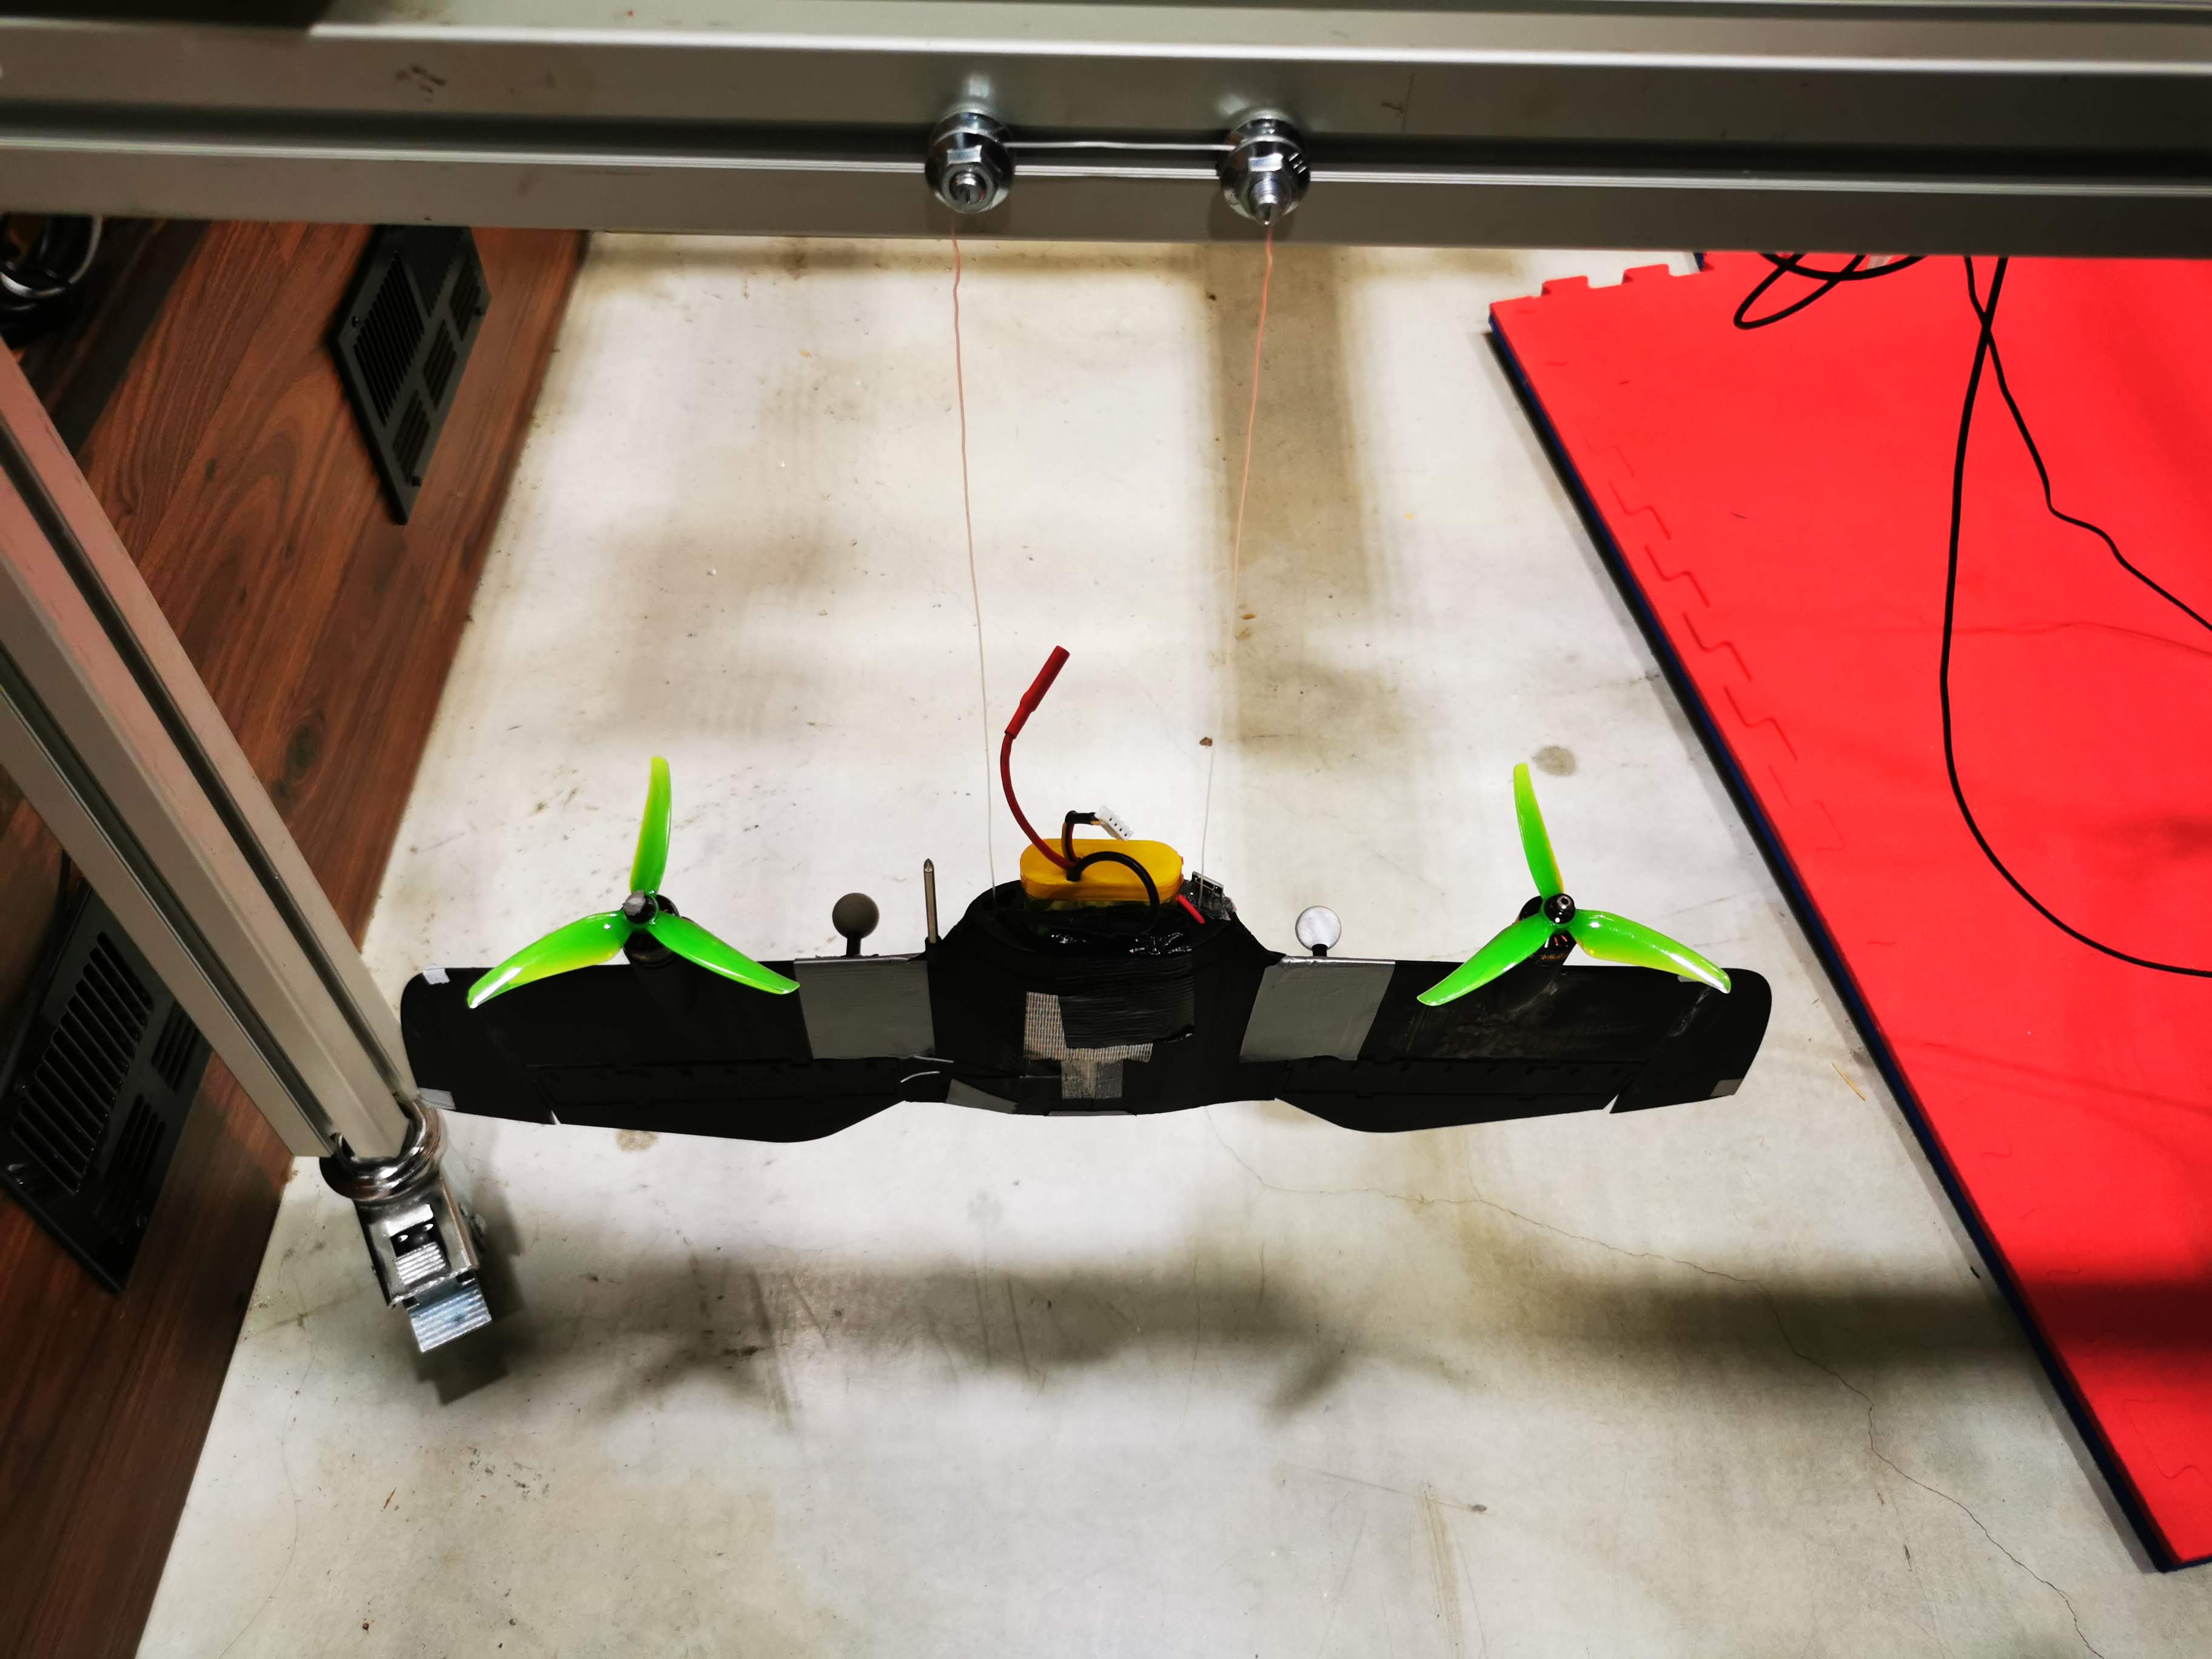
\includegraphics[trim=20cm 15cm 23cm 0cm,clip,width=0.6\columnwidth]{figures/IMG_20230609_085023.jpg}}
    \caption{Bifilar pendulum mounting for the identication of $\boldsymbol{J}$.}
    \label{fig:BifilarPend}
\end{figure}